\section{Additive Logistic Variable Selection: The ALoVaS method}

\subsection{Normal Distributions Transformed to the Unit Simplex: ALT and ALN Dynamics. }\label{sec:ALN_chapter}

This chapter outlines the additive logistic transformation, which transforms a $d$ dimensional multivariate normal distribution onto the unit simplex in $d+1$ dimensions. Note that the unit simplex in $d+1$ dimensions actually lies in a subspace of $d$ dimensions because of the constraint that the sum of the probabilities equals one. 

The goal of this chapter is to find a transform that moves the space $\mathbb{R}^d$ \newnot{symbol:real} to the simplex $\mathbb{S}^d$. \newnot{symbol:simp} The simplex $\mathbb{S}^d$ is a space defined by the constraints $\{x_i: 0<x_i<1, \sum_{j=1}^dx_j <1 \}$, and the extra term $x_{d+1}=1-\sum_{j=1}^d x_j$ ensures the total sums to 1.  

Define the notation $\yvec$, for the normal random variables that reside in the $\Rsp{d}$  dimensional space. Define the notation $\xvec$  for the vector that resides on $\simp{d}$, the simplex in $d$ dimensions. We use an underline to indicate that the stated quantity is a column vector and capital greek letters (and $I$) will denote matrices (the identity matrix) 

\begin{equation}\label{eqn:simplex_transform}
x_i = \frac{e^{y_i}}{1+\displaystyle{\sum_{j=1}^de^{y_j}}}. \\
\end{equation}
Define the Jacobian of the transformation as
\newnot{symbol:jacobian}
\begin{equation}\label{eqn:jacobian}
J(\yvec \vert \xvec) = \left( \prod_{j=1}^{d+1}x_j \right)^{-1}.
\end{equation}

It is important to note that $\yvec\in\Rsp{d}$, whereas $\xvec\in\simp{d}$. The $d$ dimensional normal has the usual parameters and density

\begin{equation}\label{eqn:multinormal}
f_{\yvec}(\yvec\vert \Sigma, \mu)=(2\pi)^{-d/2}|\Sigma|^{-1/2}\exp{\left(-1/2(\yvec-\muvec)^T\Sigma^{-1}(\yvec-\muvec)\right)}.
\end{equation}

Upon applying the transformation defined by Equation \ref{eqn:simplex_transform}, we arrive at the additive logistic normal (ALN) distribution, with density 

\begin{equation}
f_{\xvec}(\xvec\vert \Sigma, \mu)=\frac{(2\pi)^{-d/2}}{\sqrt{\vert\Sigma\vert}\prod_{j=1}^{d+1}x_j } 
\exp{\left(-1/2(\text{log}(\xvec_{(d+1)}/x_{d+1})-\muvec)^T\Sigma^{-1}(\text{log}(\xvec_{(d+1)}/x_{d+1})-\muvec)\right)}.
\end{equation}
The vector notation $\xvec_{(d+1)}$ denotes the vector in $d$ dimensions that has the $d+1$ entry removed from the vector $\xvec$. 
It is important to note that this density function is defined on the space $\simp{d}$ and \emph{not} on the space $\Rsp{d}$. 

A useful property of this transform is that we can handle probabilities defined on the $d$ dimensional simplex while working with a normal distribution. This is a common and comfortable probability distribution for most statisticians and applied scientists.
We now wish to understand how the specification of the mean vector $\muvec$ and the covariance matrix $\Sigma$ impact the structure of the ALN density. From simulation we can formulate the following conclusions: 

\begin{itemize}
\item With $\Sigma=I$, increasing the mean vector in the positive direction in any one of the $d$ components individually corresponds to shifting density towards the corner of the simplex associated with that covariate. 
\item With $\Sigma=I$, increasing the mean vector in the negative in \emph{all} $d$ components corresponds to shifting density towards the $d+1$ corner of the simplex. 
\item Keeping $\muvec =\vec{0}$, adjusting any of the variances corresponds to shifting towards a projected space of $\simp{d}$. 
\item With $\muvec =\vec{0}$, making one variance small corresponds to the shifting density towards the median of the simplex associated with the remaining $d$ dimensions. 
\item Making the $\Sigma$ matrix approximately singular and moving $\muvec$ in the negative direction for all components places most of the probability density along the median of simplex associated with first $d$ dimensions. 
\item If $\Sigma = \text{Diag}(\sigma^2_j)$,\newnot{symbol:diag} as the $\sigma^2_j$ entries become smaller, the probabilities approach the CGM specification.    
\end{itemize}

The ALN density can be simulated using the transformation defined in Equation \ref{eqn:simplex_transform} and the fact that it is easy to simulate from the vector normal distribution. 

\begin{figure}[ht]
\begin{minipage}[b]{0.45\linewidth}
\centering
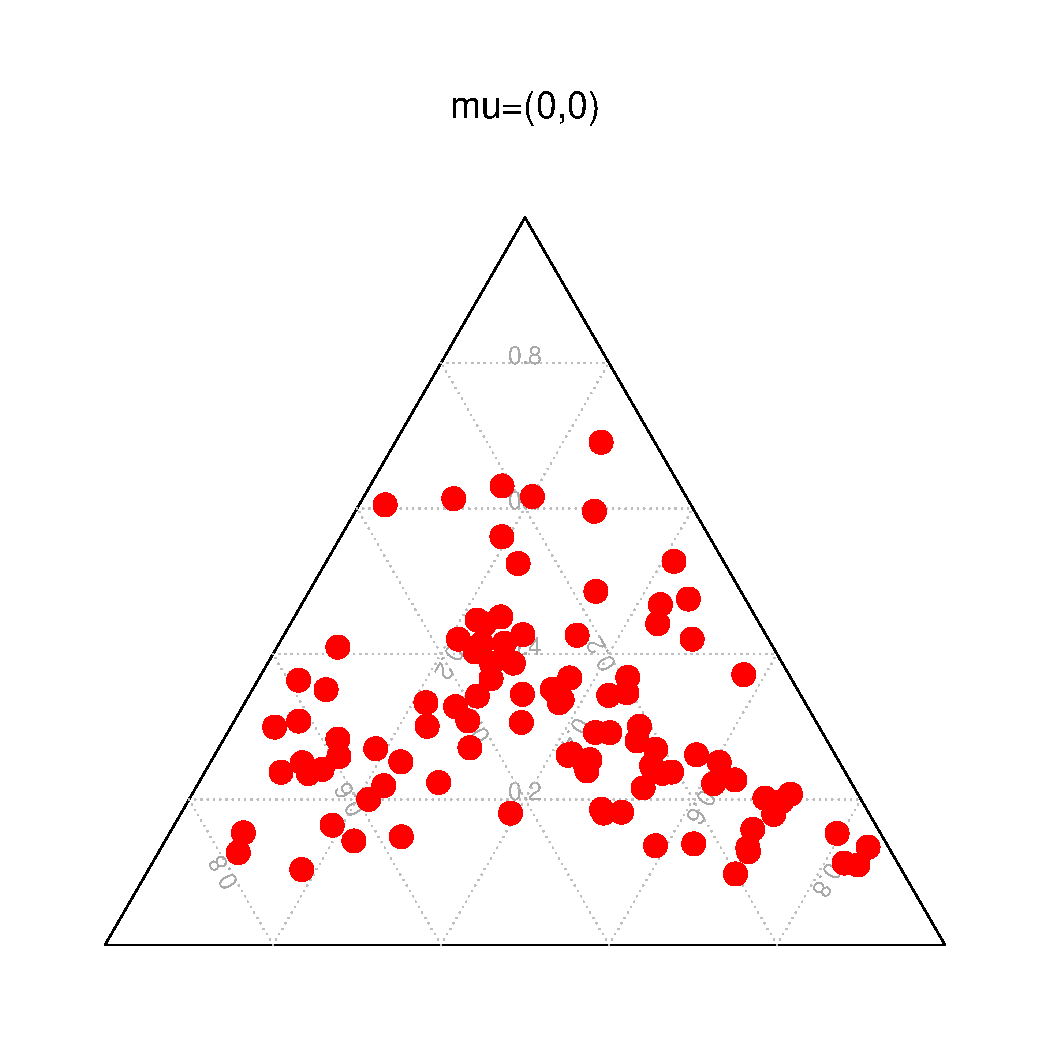
\includegraphics[width=\textwidth]{mu0_0.pdf}
\caption[ALN plot with a zero mean vector]{In this figure, $\muvec$ has all zero entries, with $\Sigma=I$, corresponding to the equiprobable case. Each probability is approximately $1/(d+1)$. }
\label{fig:figure9}
\end{minipage}
\hspace{0.5cm}
\begin{minipage}[b]{0.45\linewidth}
\centering
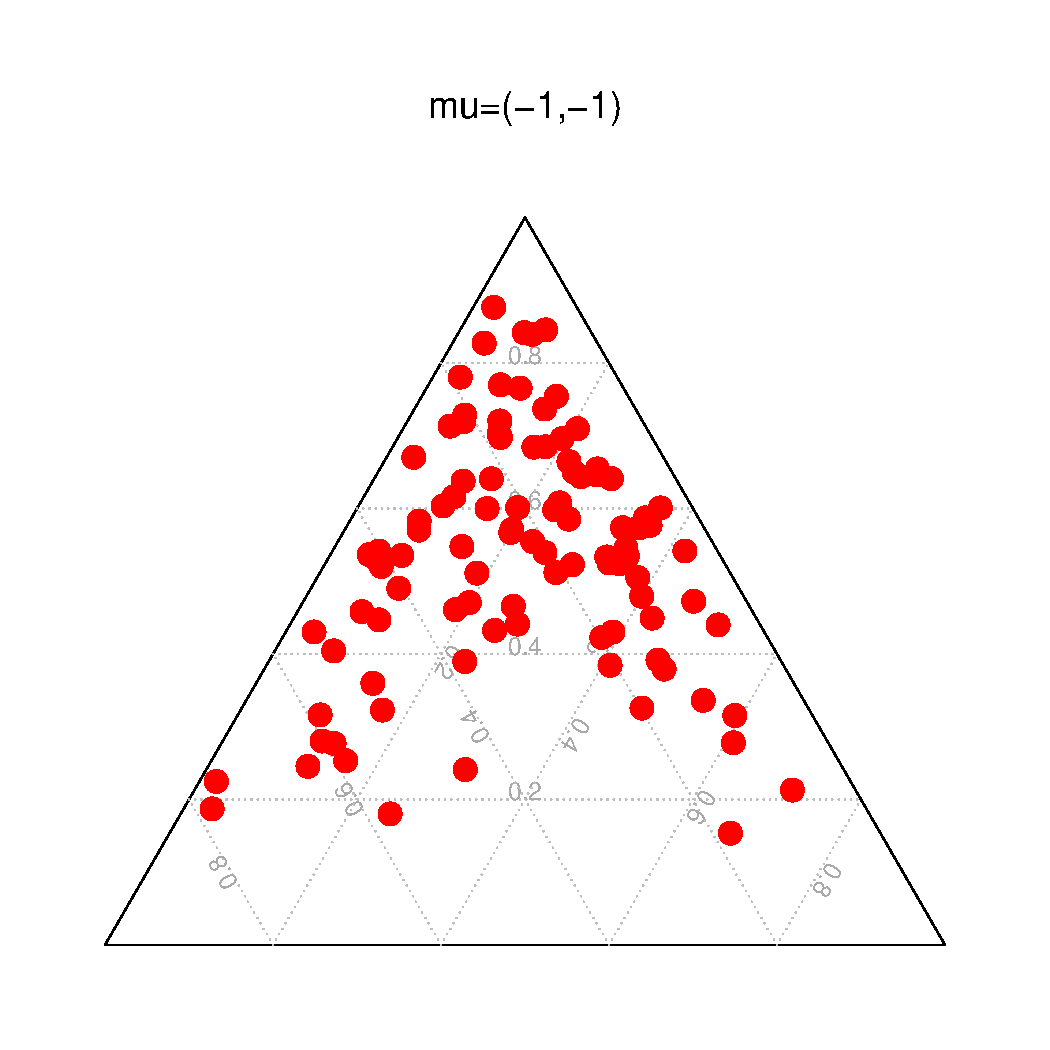
\includegraphics[width=\textwidth]{mu-1-1.pdf}
\caption[ALN plot with a negative one mean vector]{In this figure, $\vec{\mu}=(-1,-1)^T$, with $\Sigma=I$, corresponds to moving towards a sparser set of covariates. }
\label{fig:figure10}
\end{minipage}
\end{figure}

\begin{figure}[ht]
\begin{minipage}[b]{0.45\linewidth}
\centering
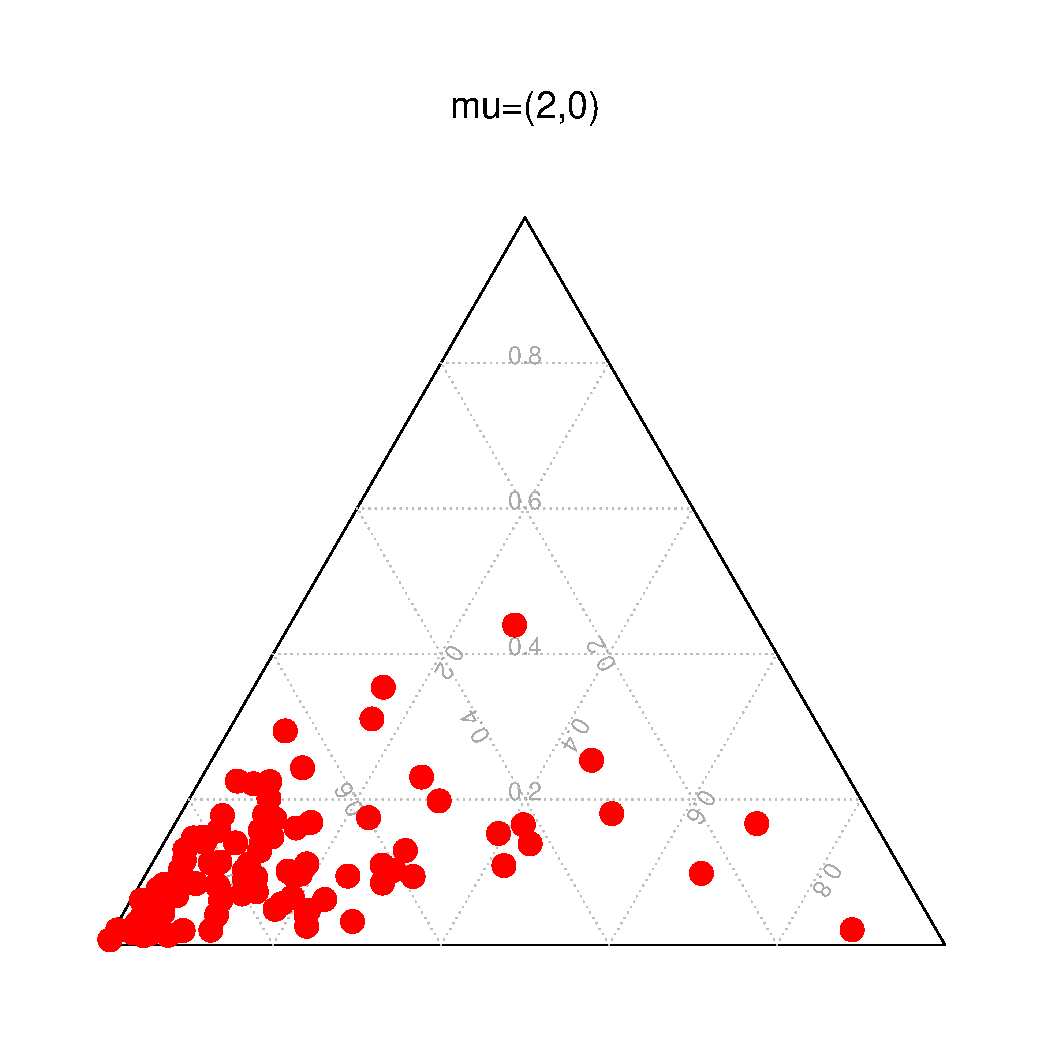
\includegraphics[width=\textwidth]{mu2_0.pdf}
\caption[ALN plot with a mean vector $(2,0)^{T}$]{$\vec{\mu}=(2,0)^T$, with $\Sigma=I$, moves the density towards one corner of the simplex. }
\label{fig:figure1}
\end{minipage}
\hspace{0.5cm}
\begin{minipage}[b]{0.45\linewidth}
\centering
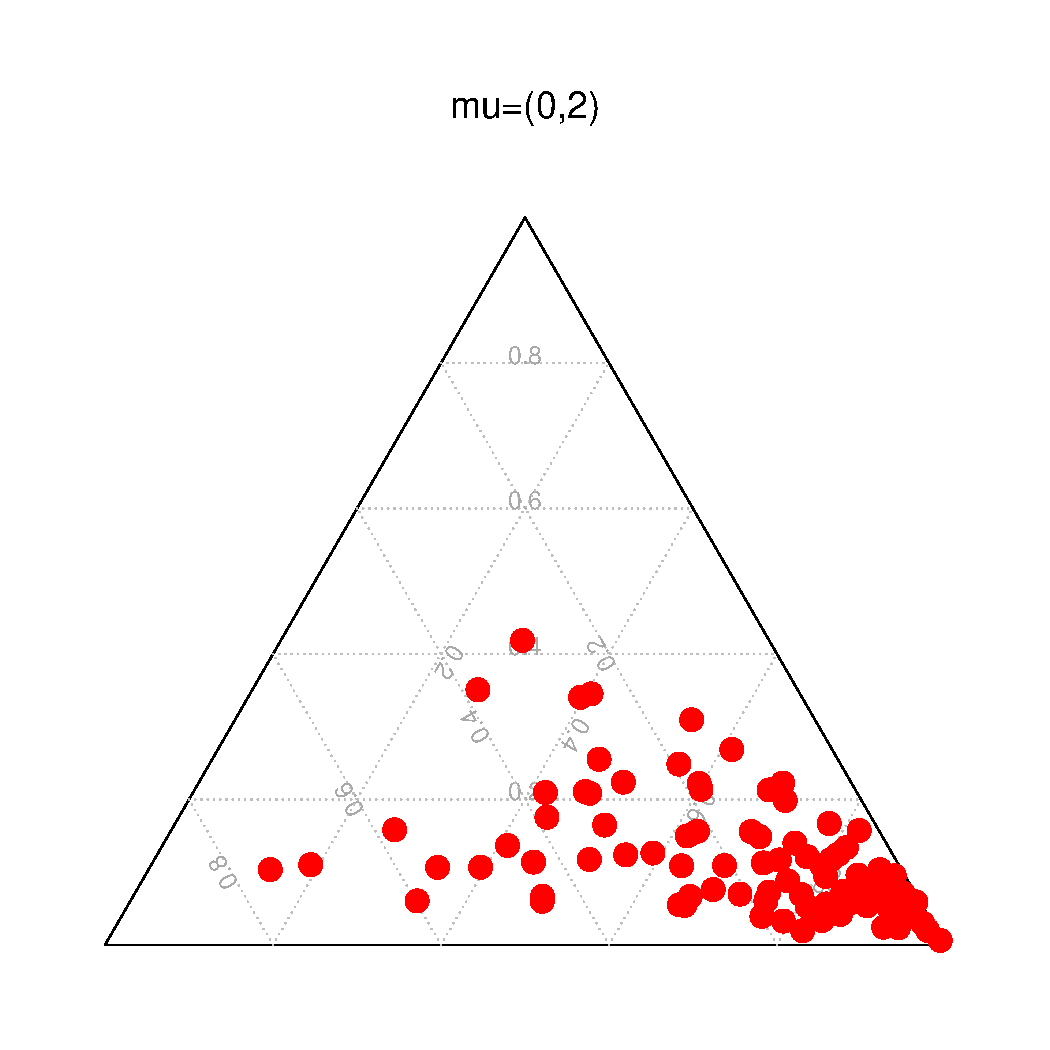
\includegraphics[width=\textwidth]{mu0_2.pdf}
\caption[ALN plot with mean vector $(2,0)^{T}$]{$\vec{\mu}=(0,2)^T$, with $\Sigma=I$, moves the density towards the other corner of the simplex. }
\label{fig:figur2}
\end{minipage}
\end{figure}

\begin{figure}[ht]
\begin{minipage}[b]{0.45\linewidth}
\centering
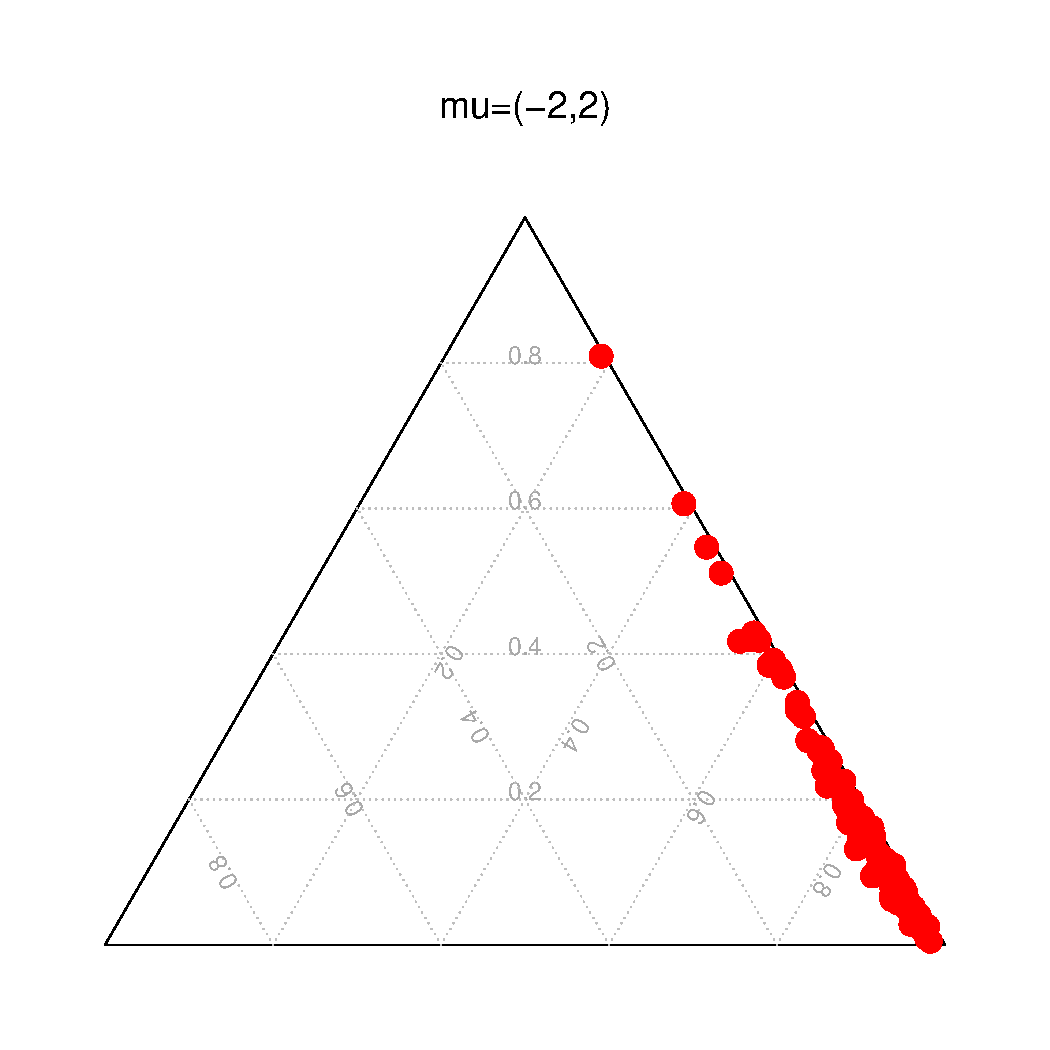
\includegraphics[width=\textwidth]{mu-2_2.pdf}
\caption[ALN plot with a mean vector of $(-2,2)^{T}$]{$\vec{\mu}=(-2,2)^T$, with $\Sigma=I$, corresponds to most probability mass along a corner of the simplex and is a sparse representation.} 
\label{fig:figure3}
\end{minipage}
\hspace{0.5cm}
\begin{minipage}[b]{0.45\linewidth}
\centering
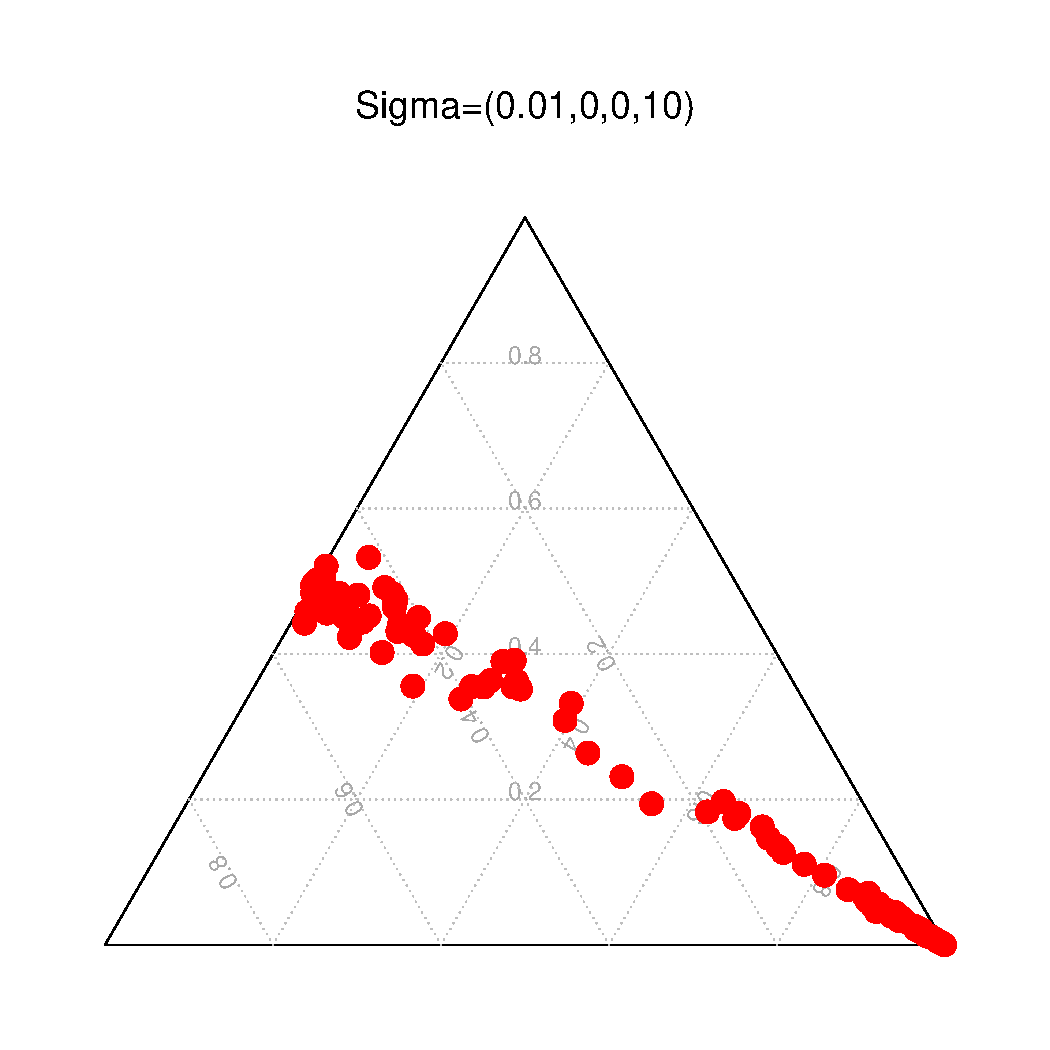
\includegraphics[width=\textwidth]{Sigma0_01_10.pdf}
\caption[ALN plot $\Sigma=\text{Diag(0.01,100)}$]{ $\vec{\mu}=\vec{0}$, with
 $\Sigma= \text{diag}(0.01, 100)$, corresponds to most density lying on a one dimensional subspace (the second covariate in the $\Rsp\ $ space).  }
\label{fig:figure4}
\end{minipage}
\end{figure}


\begin{figure}[ht]
\begin{minipage}[b]{0.45\linewidth}
\centering
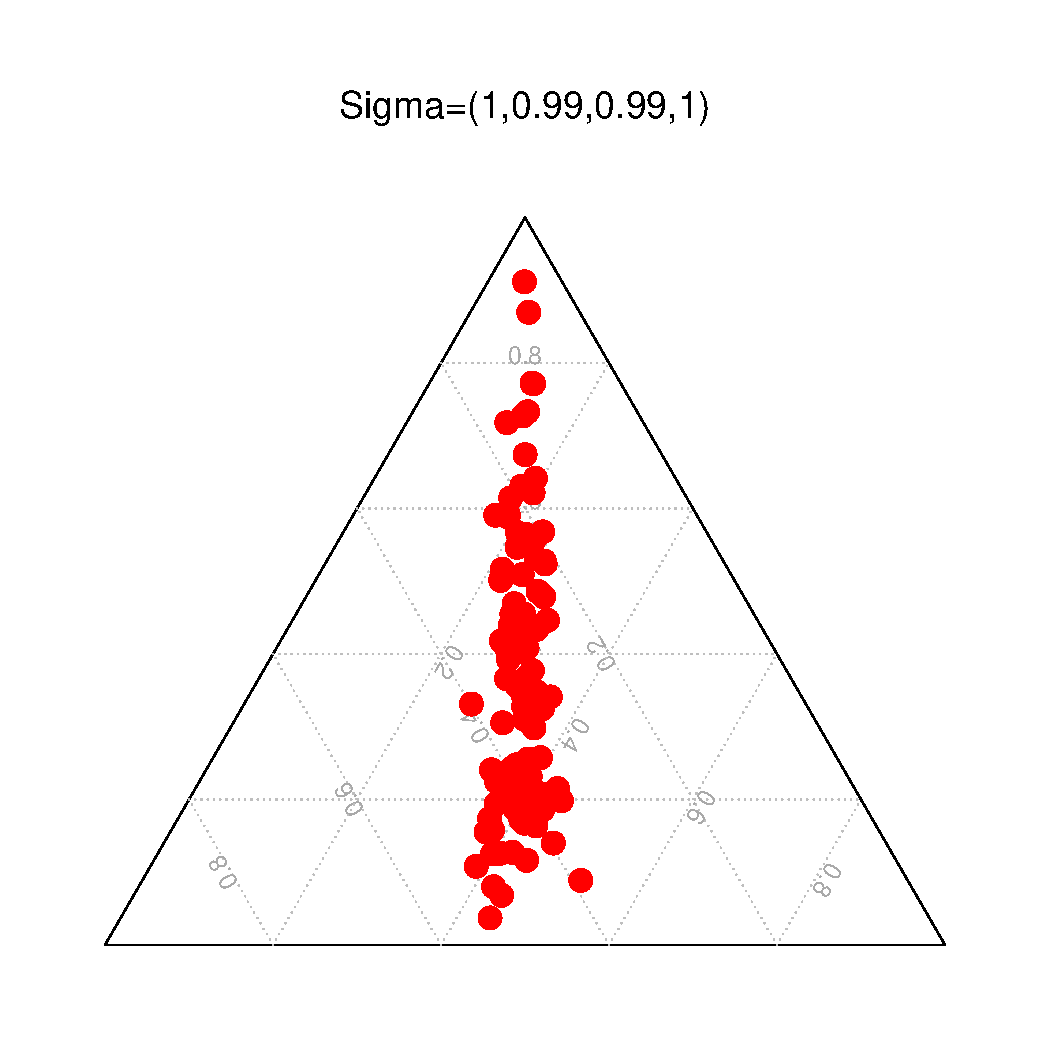
\includegraphics[width=\textwidth]{Sigma1_9_9_1.pdf}
\caption[ALN plot $\Sigma$ numerically singular]{Here $\Sigma$ is approximately singular and most of the probability mass in concentrated along the $d+1$th dimension in the $\mathbb{R}^{d+1}$ space.  }
\label{fig:figure5}
\end{minipage}
\hspace{0.5cm}
\begin{minipage}[b]{0.45\linewidth}
\centering
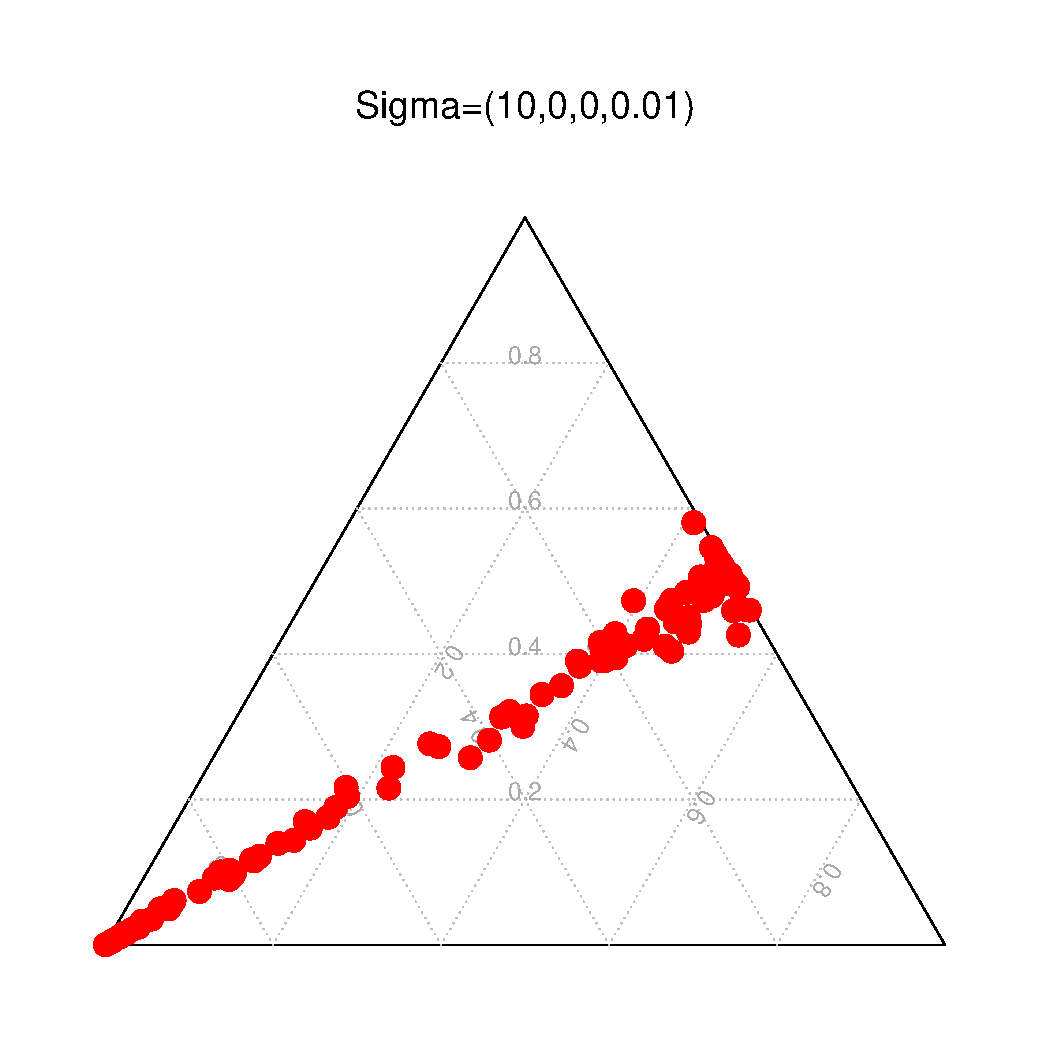
\includegraphics[width=\textwidth]{Sigma10_0_01.pdf}
\caption[Similar to the case in Figure \ref{fig:figure4} but with the variances reversed]{Similar to the case in Figure \ref{fig:figure4} but with the variances reversed.}
\label{fig:figure6}
\end{minipage}
\end{figure}

 \begin{figure}[ht]
\begin{minipage}[b]{0.45\linewidth}
\centering
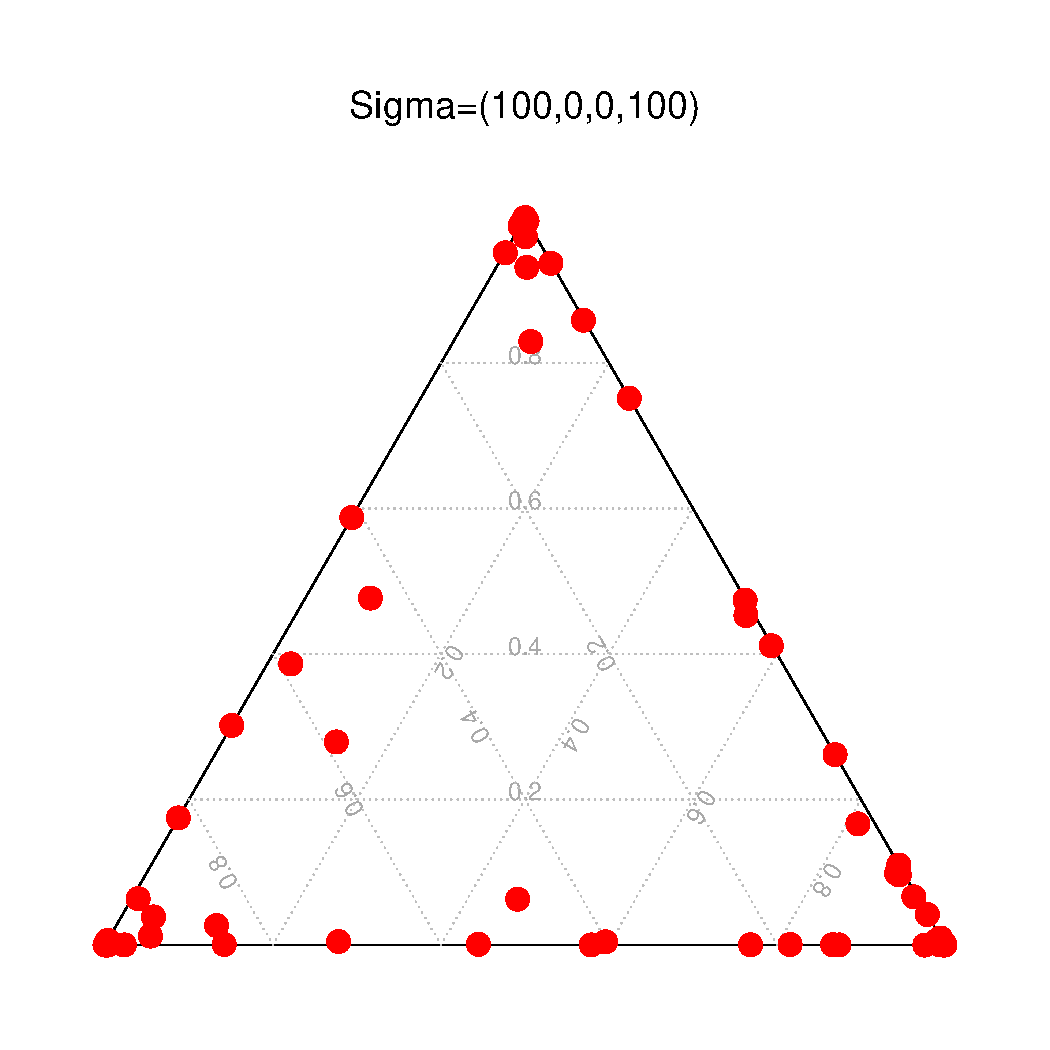
\includegraphics[width=\textwidth]{Sigma100_100.pdf}
\caption[ALN plot with a zero vector mean and $\Sigma=\text{Diag}(100,100)$]{$\vec{\mu}=\vec{0}$, with
 $\Sigma= \text{diag}(100, 100)$, corresponds to encouraging sparse representations \emph{a priori}.  }
\label{fig:figure7}
\end{minipage}
\hspace{0.5cm}
\begin{minipage}[b]{0.45\linewidth}
\centering
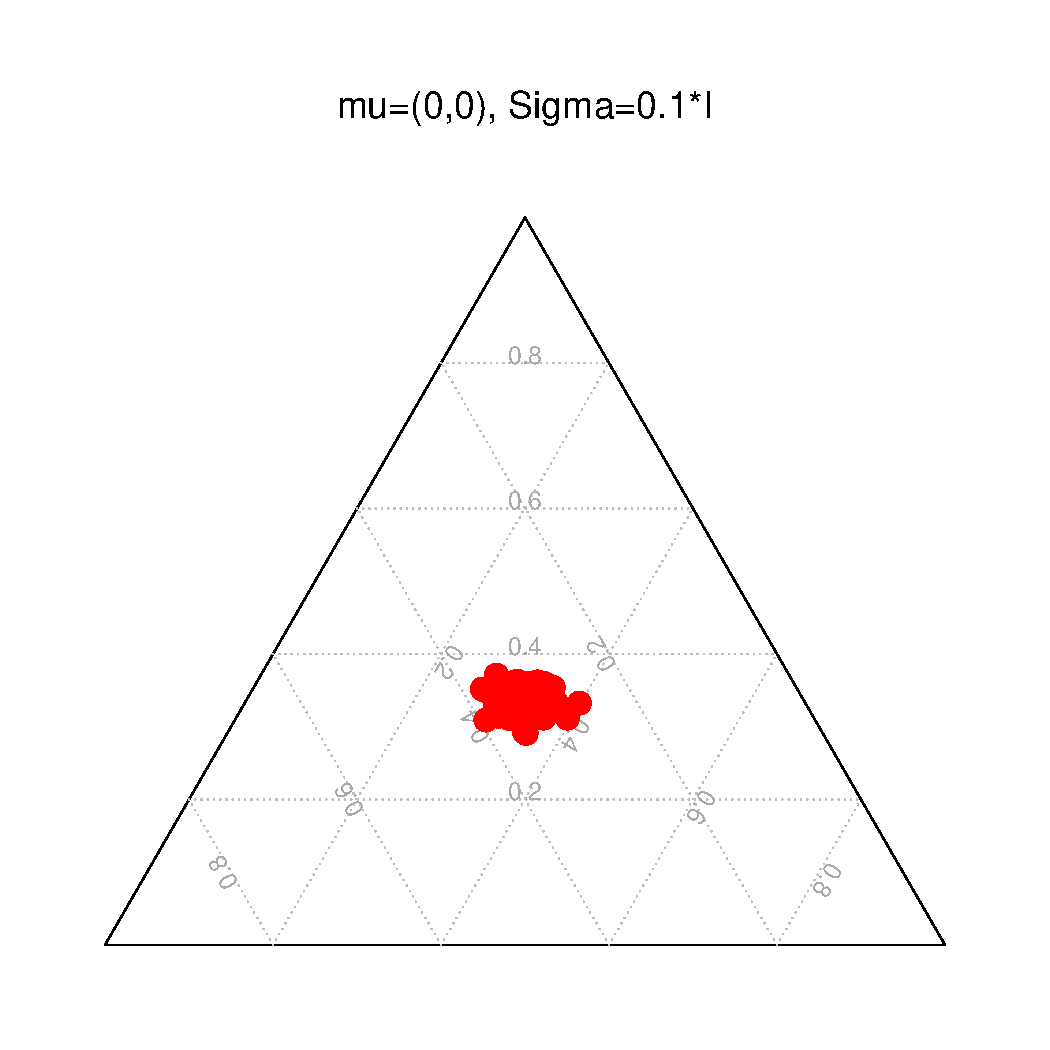
\includegraphics[width=\textwidth]{Sigma01_01.pdf}
\caption[ALN plot approximating the CGM model]{Here $\Sigma=0.1I$, and $\muvec=\vec{0}$, corresponds to roughly the CGM specification.}
\label{fig:figure8}
\end{minipage}
\end{figure}

 The simulations indicate that we can scale everything at approximately an $\mathcal{O}(d)$\newnot{symbol:big_oh} rate because of the diagonality of the variance covariance matrix, and no matrix inversions are required. The step that remains is to link this portion of the model with the (currently) observed data in the tree, so that better trees are favored over trees that are worse, when each is observed in the Markov chain. We will first work in the space $\Rsp{d}$ and then translate to probabilities by using Equation \ref{eqn:simplex_transform}.  
 
 If we focus on the means and a collection of variances in a multivariate normal i.i.d. model, then we must fully specify the likelihood and the prior to form our posterior. 
 
We define the likelihood of the tree by counting the tree's selected covariates and summing across all observed splits. The counting leads to the likelihood taking on discrete values for the observed data. Let us define a multiplier that can take on an arbitrary positive or negative value in a compact region. We then multiply the counts of splits on each covariate by this quantity, effectively creating a mean which can take arbitrary values in $\Rsp{}$. 

\subsection{A Simple Sampler Approach}

This subsection derives the full conditional densities for each necessary update in the Gibbs loop to sample posterior weights on each dimension in the CGM decision tree sampler. 
 Throughout this subsection we will use the notation $\odot$\newnot{symbol:hadamard} to denote a Hadamard product of two matrices or vectors. 
 
 \subsubsection{The General Strategy}
 There are many problems with using a Dirichlet prior and a Multinomial conjugate likelihood. The two most glaring problems are the implicit prior assumption of same scales on each covariate and the fact that all covariances or, equivalently, correlations must be negative. If the generative model of the data is a linear model with an interaction term and a decision tree model is fit to the data, then several splits will occur on the two interacting covariates. These splits will occur alternately until the curvature is sufficiently approximated \cite{ishwaran2010high}. This situation indicates a positive correlation between the two covariates. Higher order interactions will result in similar positive correlations between collections of covariates. Therefore we conclude the Dirichlet density as a posterior for the probability of selecting a covariate is an inferior model. Moreover, the initial motivation for modeling data with a decision tree was to handle survey data that contained many complex interactions that would be too computationally expensive to evaluate using linear model methods \cite{morgan1963problems}. 
 
 The likelihood will be denoted by
 
 \begin{equation}\newnot{symbol:mvn}
 MVN(\vec{c}\odot\vec{s}\vert \vec{\mu}, \Sigma=\text{Diag}(\sigma^2_j)).
 \end{equation}
 
 The prior is also a normal 
 
 \begin{equation}
 \pi(\vec{\mu}\vert \vec{\mu}_p, \Sigma)=MVN(\vec{\mu}\vert \vec{\mu}_p, \Sigma).
 \end{equation}

The priors on the variances are \iid $\sim \invgam{\sigma_j^2}{a_j}{b_j}$.
Finally the priors on the $c_j$s are \iid\ scaled beta's with densities 

\begin{equation}\newnot{symbol:scaled_beta}
S\beta(c_j\vert \alpha_j, \beta_j, -a, a)\equiv\pi(c_j\vert \alpha_j, \beta_j, -a, a)= \frac{(c_j+a)^{\alpha_j-1}(a-c_j)^{\beta_j-1}\Gamma(\alpha_j+\beta_j)}{(2a)^{\alpha_j+\beta_j-1}\Gamma(\alpha_j)\Gamma(\beta_j)}.
\end{equation}

A special case of these scaled beta densities is when $\alpha_j=\beta_j=1$, which yields uniform r.v.'s on the region  $[-a,a]$. 
For each $j=1, \dots, d$, we first calculate $s_j = \epsilon+\sum_{\forall \eta \in \mathcal{T}}\mathds{1}[\text{split on covariate j at node $\eta$}]$, for some fixed $\epsilon>0$.
Through basic Bayesian calculations we find that the full conditional distributionss are 

\begin{equation}
\pi(c_j\vert \mu_j, \sigma_j^2, a) \sim N_{[-a,a]}(c_js_j\vert \mu_j, \sigma^2_j) \text{(a normal truncated to the region $(-a,a)$),}
\end{equation}

\begin{equation}
\pi(\sigma^2_j \vert \mu_j, c_j, a) \sim \invgam{\sigma_j^2}{2a_j+2}{\frac{(c_js_j-\mu_j)^2+ (\mu_j-\mu_j^p)^2+b_j}{2}}, \text{ and } 
\end{equation}

\begin{equation}
\pi(\mu_j\vert \mu_j^p, c_j, \sigma^2_j)\sim N[c_js_j+\mu_j^p, \sigma_j^2].
\end{equation}

\subsection{Slice Sampling Gibbs Updates}

Ideally we would like everything to be a Gibbs step. This can be accomplished numerically using numerical approximations to the cumulative density of the standard normal distribution, here denoted $\Phi$, and $\Phi^{-1}$, the quantile function of the standard normal cumulative density. \newnot{symbol:sncdf} However, we can accomplish this directly using the technique of parameter expansion set forth in Damien and Walker \cite{damien2001sampling}, which we review here for completeness. 
 
We begin with the joint density of two random variables 

\begin{equation}
f(x,y) \propto \mathds{1}[0, \exp{(-x^2/2)}](y).
\end{equation}
The marginal of $x$ is a standard normal density. Through elementary probability calculations we find 

\begin{equation}\newnot{symbol:unif}
f(y\vert X=x) \propto Unif(0, \exp{(-x^2/2)}),
\end{equation}
 and 
 
 \begin{equation}
f(x\vert Y=y) \propto Unif(-\sqrt{-2log(y)}, \sqrt{-2log(y)}).
\end{equation}
The region upon which $X$ is defined arises from the solution of the inequalities $\{0\leq y \leq \exp{(-x^2/2)} \} $ for $X$, which is a quadratic equation in $X$. Similarly, if we have a truncated distribution truncated to the region $[a,b]$, we write the joint density 
 
 \begin{equation}
 f(x,y)=Unif((0\leq y\leq \exp{(-x^2/2)})\times (a,b)).
 \end{equation}
 Solving the resulting system of inequalities leads to the set 
 
 \begin{equation}
 \{-\sqrt{-2log(y)}, \sqrt{-2log(y)} \} \cap \{a, b\},
 \end{equation}
which results in the region for $x$

\begin{equation}
 \{\text{max}(a,-\sqrt{-2log(y)}), \text{min}(b,\sqrt{-2log(y)} )\} .
 \end{equation}
 Simulating from a truncated normal is equivalent to simulating from two uniforms on the appropriate regions and evaluating a natural logarithm and a square root function at each iteration. 
 
 A special case of these scaled beta densities is when $\alpha_j=\beta_j=1$, which yields uniform random variables on the region $[-a,a]$. 
For each $j=1, \dots, d$, we first calculate $s_j = \epsilon+\sum_{\forall \eta \in \mathcal{T}}\mathds{1}[\text{split on covariate j at node $\eta$}]$, for some fixed $\epsilon>0$.
Through basic Bayesian calculations we find the full conditionals in closed form
 
\begin{equation}\label{eqn:u_given_cjsj}
\pi(u \vert c_js_j, \mu_j, \sigma_j^2)= \text{Unif}(0, \exp{(\frac{-(c_js_j-\mu_j)^2}{2\sigma_j^2} )}),
\end{equation}

\begin{equation}
\pi(c_j \vert u) = \text{Unif}(\text{max}(-a,-\sqrt{-2log(u)}), \text{min}(a,\sqrt{-2log(u)} )),
\end{equation}

\begin{equation}
\pi(\sigma^2_j \vert \mu_j, c_j, a) \sim \invgam{\sigma_j^2}{2a_j+2}{\frac{(c_js_j-\mu_j)^2+ (\mu_j-\mu_j^p)^2+b_j}{2}}, \text{ and}
\end{equation}

\begin{equation}\label{eqn:muj_given_cj}
\pi(\mu_j\vert \mu_j^p, c_j, \sigma^2_j)\sim N[c_js_j+\mu_j^p, \sigma_j^2].
\end{equation}

 The Gibbs sampling step, nested within the MH sampler, proceeds by sampling from Equations \ref{eqn:u_given_cjsj}-\ref{eqn:muj_given_cj}.
At each iteration, once samples are drawn in sequence from the distributions given in Equations \ref{eqn:u_given_cjsj}- \ref{eqn:muj_given_cj}, we take the posterior samples of $\mu_j$ and transform these onto the $[0,1]$ scale, by using the ALN transform given in Equation \ref{eqn:simplex_transform}. 

We show results from a preliminary coding of the stated algorithm. We use two specificications for the prior means $\vec{\mu}^p$. One specification uses  $\vec{\mu}^p = \vec{0}$ (Figure \ref{fig:simple_sampler2}) and another uses $\vec{\mu}^p=(-2,-2,2,\dots,2)$ (Figure \ref{fig:simple_sampler1}). The difference in the results of sampled weights indicates that, if we can move from a negative to a positive value for the prior mean, we can greatly influence the selection of covariates. The graphic of posterior weights shown in Figure \ref{fig:simple_sampler1} is the correct set of weights for the data. 


%%%% -------Graphics from preliminary simulations using the simple sampler approach

 \begin{figure}[ht]
\begin{minipage}[b]{0.45\linewidth}
\centering
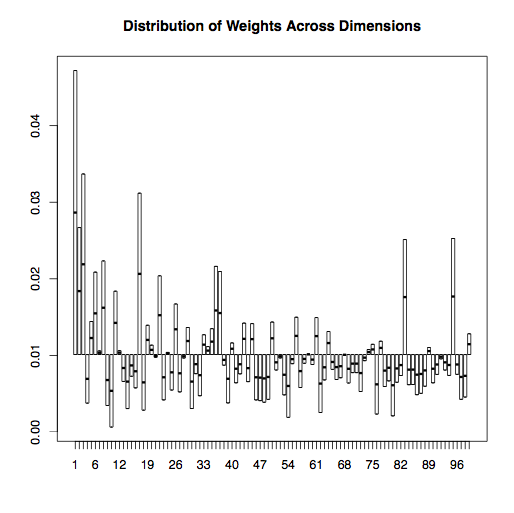
\includegraphics[scale=0.4]{simple_sampler2.png}
\caption[Results for the zero mean prior]{A zero mean prior. Note that the two covariates that should have large probabilities are covariates 1 and 2.}
\label{fig:simple_sampler2}
\end{minipage}
\hspace{0.5cm}
\begin{minipage}[b]{0.45\linewidth}
\centering
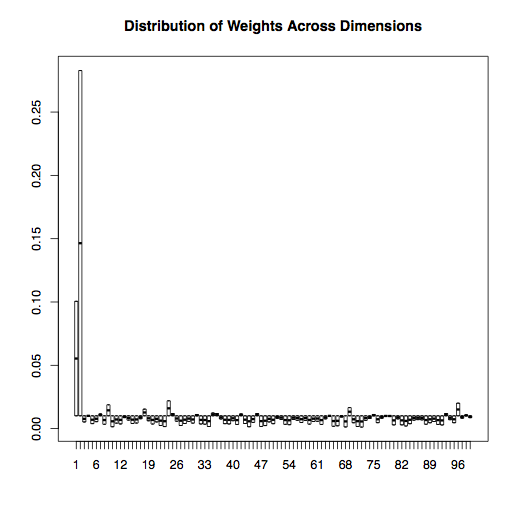
\includegraphics[scale=0.4]{simple_sampler1.png}
\caption[Results for the informative prior]{An informative prior. The first two prior means are 2 and the remaining prior means are set at -2.}
\label{fig:simple_sampler1}
\end{minipage}
\end{figure}


%%%%---------END OF: Graphics from preliminary simulations using the simple sampler approach

\subsection{A Stochastic Search Variable Selection Approach}

Using the results of George and McCulloch we derive Gibbs updates for each of the parameters and have as a special case the approach of CGM if all the dimension indicators are selected to be the point masses at zero. In this case the ALN transform puts probability $1/(d+1)$ on each dimension. 


We investigate three priors for use in variable selection with decision trees. They are: 

\begin{itemize}
\item A stochastic search approach using method of George and McCulloch \cite{cui2008empirical,george1993variable}. 
\item A lasso prior on the means of the MVN, \newabbrev{abbrev:MVN} using parameter expansion to use Gibbs updates \cite{park2008bayesian}. 
\item A multivariate half-Cauchy prior using parameter expansion (Huang and Wand method) \cite{huang2013simple,polson2011half,carvalho2010horseshoe,carvalhohandling}. 
\end{itemize}

We will discuss the preliminary details of each method in sequence in this chapter. 

Variable selection with SSVS facilitates a Bayesian approach to variable selection in decision trees. Prior methods have examined bootstrapping approaches and used some complicated math to allow the statistician to peer inside the black box method known as randomForest \cite{ishwaran2010high, ishwaran2007variable}, often with little insight or understanding. The SSVS prior allows us to ``test'' whether the constant prior probability of selecting a covariate for all dimensions is appropriate for the given dataset. This means we can test, for any dataset, whether the CGM model of covariate selection is appropriate.

%We will implement and compare our method against other methods such as observed frequency, a na\"{i}ve method, as well as the maximal subtree approach of Ishwaran et al. \cite{ishwaran2010high, ishwaran2007variable}. The SSVS approach involves a prior on the normal means of the form 

\begin{equation}
\pi(\mu_i\vert \tau_i, p_i, c_i) \propto p_iN(\mu_i, \tau_i^2)+(1-p_i)N(\mu_i, \psi^2_i+\tau_i^2).
\end{equation}

Here the $\psi_i >0$ and the $\tau_i>0$. Usually $p_i\equiv1/2$ but it is also possible to put a prior on these hyper-parameters. The advantage of a mixture prior in this form is that Gibbs samples are readily available for each of the desired quantities facilitating fast sampling.     

\subsection{Parameter Expansions For the Lasso and Horseshoe Priors}
In this section we propose to use parameter expansion to facilitate Gibbs sampling within the sampling framework for the posterior means ($\mu_j$) for each covariate in the normal space. We use the ALN transform to convert the $\mu_j$ to probabilities using the ALT transform. 
We use the scale mixture of normals representation to write the Laplace prior is parameter expanded form. This representation is stated here for reference.

If $V \sim \text{Exponential(1)}$ and $Z \sim N(0, 1)$ independent of $V$, then $X = \mu + b \sqrt{2 V}Z \sim \mathrm{Laplace}(\mu,b)$. 

Equivalently we can write this as the hierarchy

\begin{equation}\label{eqn:normal_cond_lhood_lasso}
X \vert V \sim N[\mu, \sigma^22V],
\end{equation}

\begin{equation}\newnot{symbol:exponential_dist}
V \sim \text{Exponential}(1), \text{ and}
\end{equation}

\begin{equation}\newnot{symbol:laplace_dist}
X \sim \text{Laplace}(\mu, \sigma).
\end{equation}

What we want to examine here is whether shrinkage along an $L_1$ penalty will achieve similar results to the SSVS approach and give us meaningful results. The belief here is the same as in the SSVS approach, shrinkage will shrink means toward zero in the multivariate normal. These sampled values from the multivariate normal will then be transformed into something on the $[0,1]$ (probability) scale using the ALN transform. Values of zero, or near zero, on the normal space transform into values of approximately $1/(d+1)$. The probabilities with values around $1/(d+1)$ correspond to covariates we are indifferent about. A confounding aspect of interpreting the probabilities is that they must all sum to 1. Therefore if some values are excessively small this may push all the other probabilities to be larger. If something like this happens it is then difficult to determine which covariates are non-informative. Further simulations regarding selecting covariates using the rule of Equation \ref{eqn:cov_inclusion_rule} will be conducted using the ALN transform and will be done on several simulated and real data examples.    

The following result will be useful for parameter expansion. If 

$X\vert a \sim \mathrm{Inv\textendash Gamma}(\nu/2, \nu/a)$ and  $a \sim \mathrm{Inv\textendash Gamma}(1/2,A^2)$, then $\sqrt{X}\sim \mathrm{Half\textendash Cauchy}$. 

\begin{align*}
f(x) &= \int_0^\infty \underbrace{  \frac{\nu^{\nu/2}}{a^{\nu/2}\Gamma(\nu/2)x^{(\nu/2)+1}}\exp{(-\frac{\nu}{ax})}   }_{=f(x\vert a)} \underbrace{\frac{\exp{(-\frac{1}{aA^2})}}{A\sqrt{\pi}a^{3/2}}}_{=f(a)} da\\
&=\frac{\nu^{\nu/2}}{A\sqrt{\pi}\Gamma(\nu/2)x^{(\nu+2)/2}}\underbrace{\int_0^\infty a^{-\nu/2-1/2-1}\exp{(-(1/a)(\nu/x+1/A^2))}da}_{=\text{Inv-Gamma kernel}}\\
&=\frac{\nu^{\nu/2}\Gamma((\nu+1)/2)}{A\sqrt{\pi}\Gamma(\nu/2)x^{(\nu+2)/2}(\nu/x+1/A^2)^{(\nu+1)/2}}\\
&\propto \frac{1}{\sqrt{x}x^{(\nu+1)/2}(\nu/x+1/A^2)^{(\nu+1)/2}}\\
& =\frac{1}{\sqrt{x}(\nu+x/A^2)^{(\nu+1)/2}  }\\
&=\frac{1}{\sqrt{x}(\nu+x/A^2)^{(\nu+1)/2}  }.
\end{align*}

Making the change of variable $x=y^2$, which implies $dx/(2\sqrt{x})=dy$, shows us that 

\begin{equation}
f(y) \propto (1+(y/A)^2/\nu)^{-(\nu+1)/2},
\end{equation}
for $y>0$ which is the definition of a half-Cauchy density. 

Huang and Wand \cite{huang2013simple} indicate that using an inverse-Wishart prior on the variances, with each standard deviation having a half-Cauchy prior, gives a scaled beta marginal for each correlation. At this point it is worth recalling that the t and half-t distributions have as special cases, the Cauchy and half-Cauchy distributions when the degrees of freedom parameter ($\nu$) in the t and half-t is set to $\nu=1$. 



\section{The ALoVaS Model}\label{sec:Introduction}
	
In this paper we describe a decision tree method to explicitly handle variable selection in high-dimensional data, called the Additive Logistic Variable Selection  (ALoVaS) method. This method allows us to reuse regularization approaches, prominent in the linear model literature, and apply them to decision trees. Although Bayesian methods have been available for use with decision trees since the seminal papers of Chipman, George, and McCulloch \cite{chipman1998bayesian}  and Denison, Mallick, and Smith \cite{denison1998bayesian}, there has been little work to alleviate the practical difficulties of applying Bayesian decision trees for high-dimensional data. A notable exception is the approach of Roberts and Leman \cite{Roberts:2013uq} who used a Dirichlet prior on the covariate selection probabilities. Also, the non-Bayesian approaches described by Ishwaran and coauthers \cite{ishwaran2011random,ishwaran2010high,ishwaran2007variable} deserve mentioning these authors use an initial bootstrap sample to determine the covariate selection probabilities and then use these estimated covariate selection probabilities in a subsequent random forest algorithm. Moreover, in the discussion of Chipman et al., it is noted by Knight, Kustra, and Tibshirani \cite{knight1998bayesian} that the Bayesian approach to decision trees breaks down as the number of covariates increases. 

In contrast to the literature on decision tree variable selection, the literature on variable selection for linear models is voluminous. Textbooks have been written on variable selection for linear models \cite{miller2002subset}. Each year several papers are published in major statistical journals developing properties of various variable selection methods and proposing modifications to improve known deficiencies. 

Let us start with the linear model
\begin{equation}\label{def:linear_model}
\vec{y} = X\vec{\mu} + \vec{\epsilon},
\end{equation}
where $\vec{\epsilon}$ is an $n \times 1$ vector of random errors, typically assumed to follow a multivariate normal distribution. Also, $X$ is an $n \times p$ matrix, also called the design matrix, which determines the mean value associated with each observed response, the associated element of the $n\times 1$ vector $\vec{y}$. It should be noted that in this section and throughout this paper we use the cell means model to describe the ANOVA linear model. Thus here $X$ denotes an incidence matrix of full rank. It is well known that if $n$, the number of observations, is less than $p$, the number of covariates, then the estimated values of the $\mu_j$, for $j=1,\dots,p$, denoted $\hat{\mu}_j$, are not estimable. However, regularizing, or equivalently putting a prior on the $\mu_j$, results in estimable values for the $\hat{\mu}_j$. Moreover, a nice property of the linear model is that covariates deemed not useful can have their coefficients coded as zero, whereas useful covariates can be encoded with non-zero coefficients. Thus, a sparse linear model indicates knowledge that certain covariates are not useful. Sparse linear models are typically necessary when dealing with high-dimensional data, especially in the $p>n$ case. 

The Additive Logistic Transform (\ALT), when employed with a multi-category logistic regression, is used as the canonical inverse link function \cite{mccullagh1989generalized}. The \ALT\ is referred to as the softmax function in the machine learning literature \cite{bishop2006pattern}. Additionally, the \ALT\ is fundamental to the analysis of compositional data \cite{aitchison1986statistical}. The \ALT\ is defined by the vector valued function given in Equation \ref{eqn:alt}, 
\begin{equation}\label{eqn:alt}
\vec{q} = \left[ q_1, q_2,\dots, q_{p-1}, q_p \right] =\vec{g}^{-1}(\vec{\mu})= \left[ \frac{e^{\mu_1}}{1+S_{p-1}},\frac{e^{\mu_2}}{1+S_{p-1}}, \dots,\frac{e^{\mu_{p-1}}}{1+S_{p-1}},\frac{1}{1+S_{p-1}} \right],\end{equation} 
where $S_{p-1}=\sum_{j=1}^{p-1}e^{\mu_j}$. Moreover, the \ALT\ is an invertible mapping from the $p$ dimensional real number system to a probability simplex. This allows us to calculate the distribution of the random variables obtained by the \ALT\ via a change of variables. In this paper we focus on the Additive Logistic Normal (\ALN) density, obtained by applying the \ALT\ to a random vector with a multivariate normal density. The \ALN\ density has proved successful in the correlated topic model \cite{blei2007correlated,lafferty2005correlated}.  Additionally, for our applications the \ALN\ density allows us to model covariate selection probabilities that have both positive and negative correlations, whereas distributions like the Dirichlet density only permit negative correlations.

By focusing on the \ALT, we are able to transform the decision tree variable selection problem into a problem of variable selection in a linear model. The upshot of this is that we may use variable selection methods, prevalent in the linear model literature, with decision trees. Thus, we can sample from a posterior distribution of the covariate selection probabilities and determine the utility of covariates, simultaneously performing variable selection and decision tree fitting. 
 
\begin{figure}[H]
  \centering
  \begin{tabular}{ccc}
 \subfigure[]
 {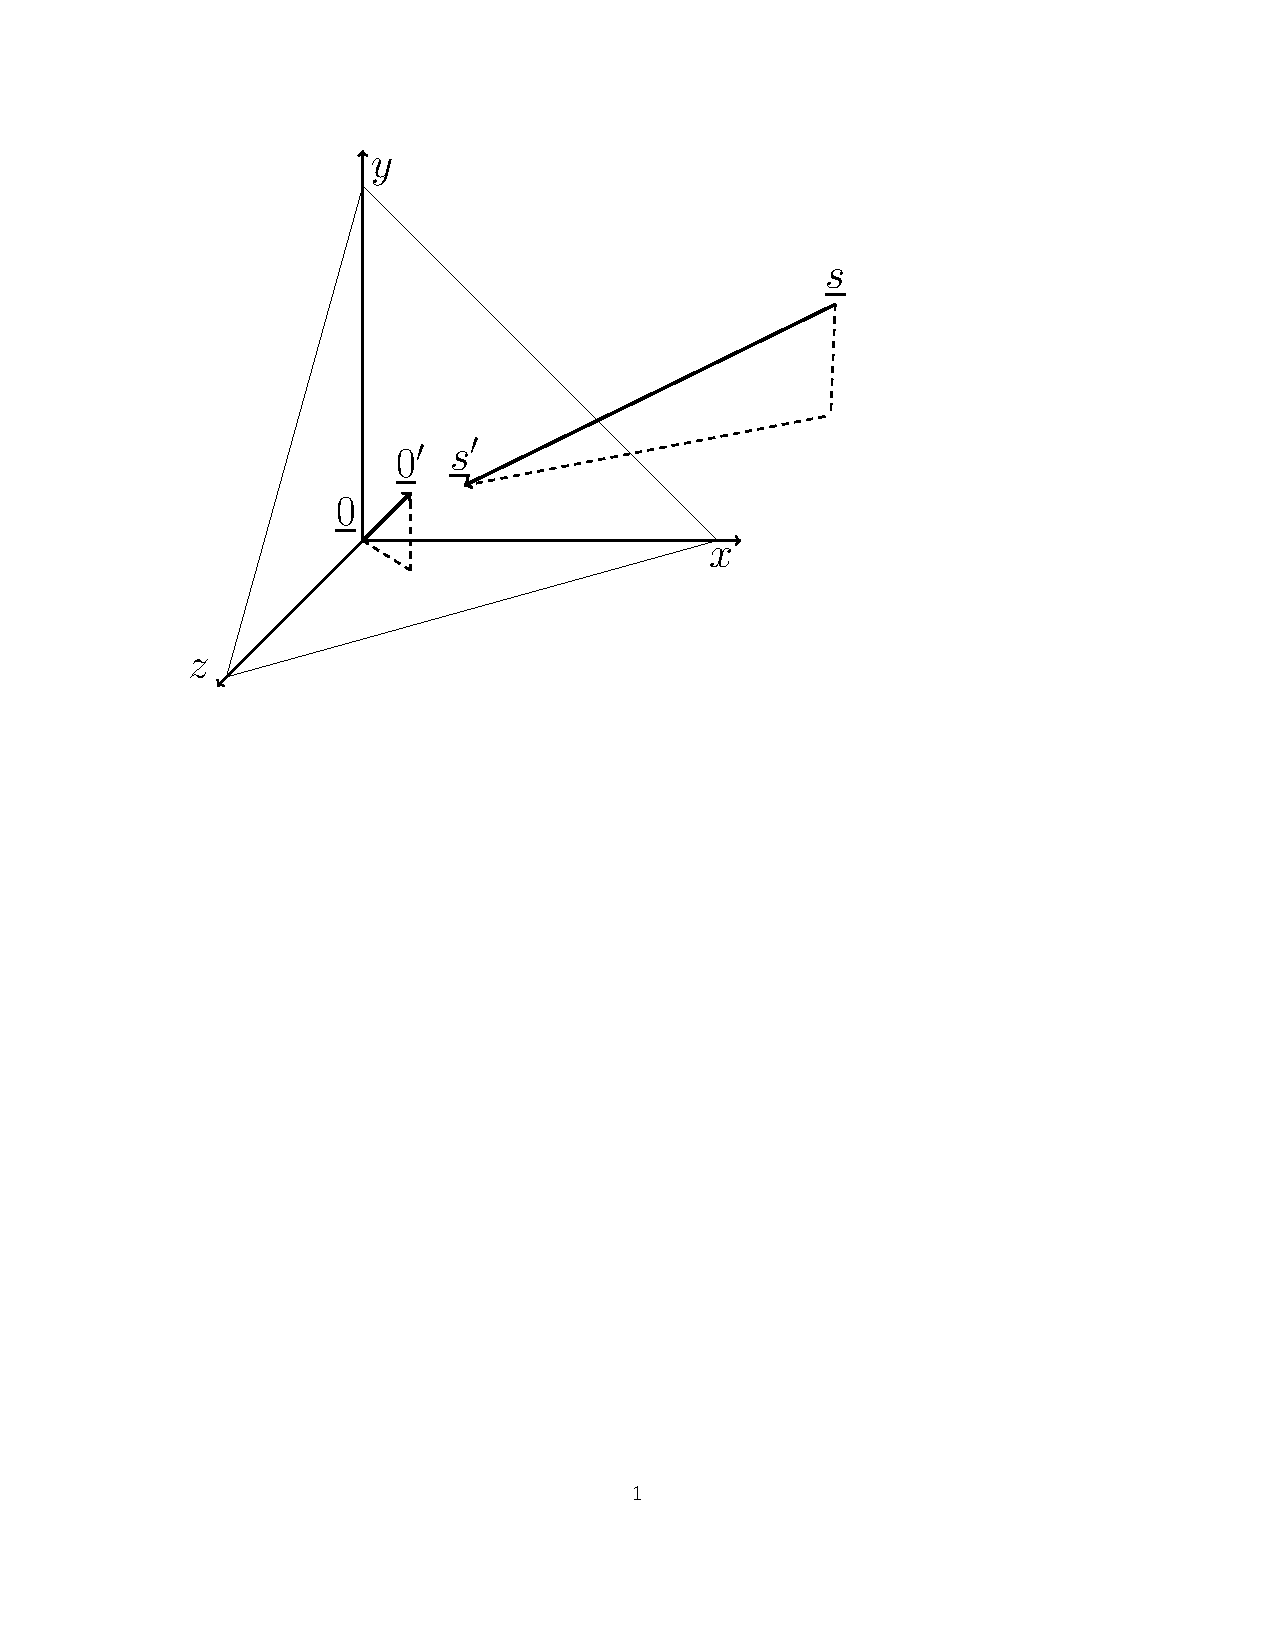
\includegraphics[trim={3cm 16cm 5cm 1cm},clip,scale=0.5]{figures/prob_plot_tikz_bw.pdf}}
%    & \num\putindeepbox[2pt]{\includegraphics[scale=0.25]{figures/real_space_tikz.png}} 
    & \subfigure[]{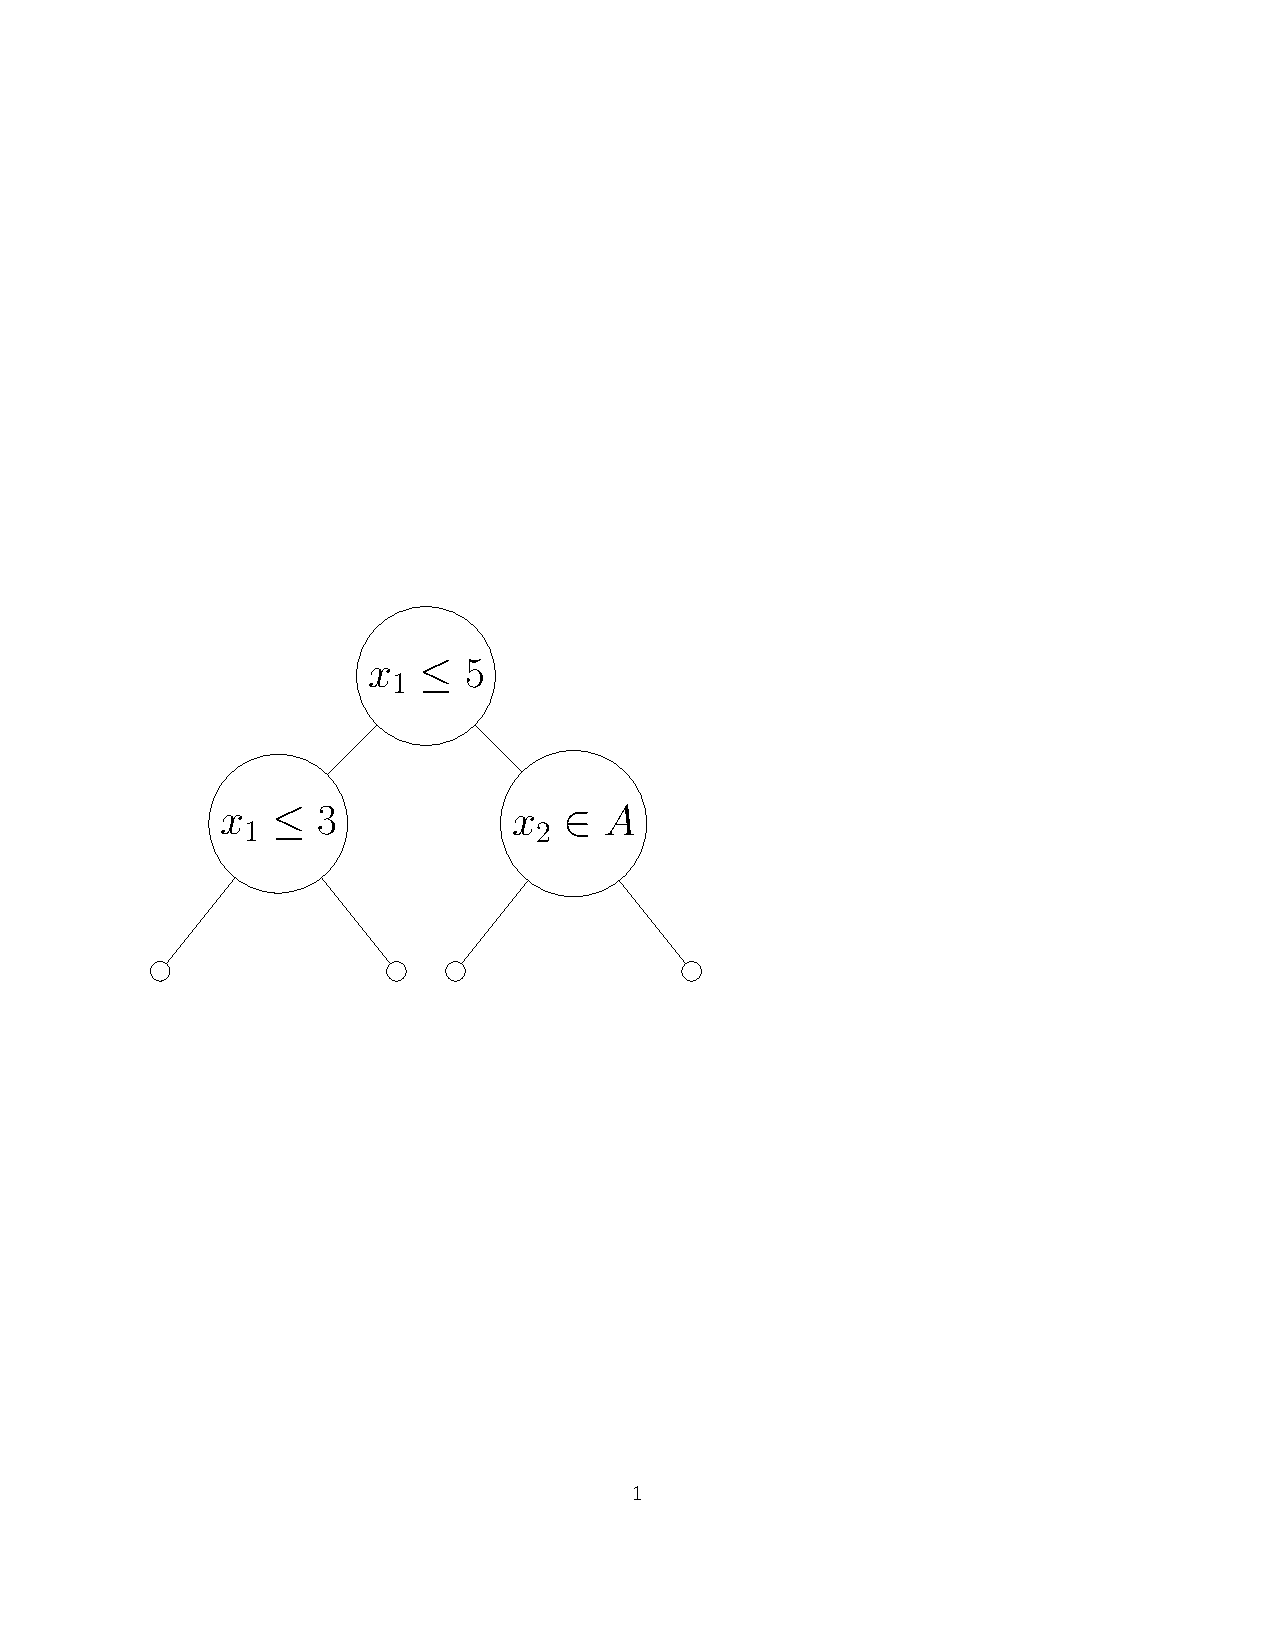
\includegraphics[trim={2cm 11cm 8cm 10.1cm},clip,scale=0.7]{figures/simple_tree_tikz.pdf}} \\
\end{tabular}
  \caption{In (a) we plot the points in the Euclidean space and the primed points represent the points mapped to the probability simplex, represented in the plot by the surface of the triangular plane given by the equation $x+y+z=1, x,y,z >0$. The primes indicate points on the probability simplex after applying the additive logistic transformation to the split counts. In (b) we plot an example decision tree splitting on two of three possible covariates.}
  \label{fig:trees_and_probability}
\end{figure}
 
 Consider Figure \ref{fig:trees_and_probability}; in this figure we have a plot of a decision tree and a plot of the probabilities associated with the tree on a two-dimensional simplex and the three-dimensional Euclidean space. If the observed data has only three covariates and we only observe the first two covariates, $x_1$ and $x_2$ in the estimated tree, then the covariate selection probability vector is approximately $\vec{p} = [0.50, 0.31, 0.19]$. The covariate that has no observed splits receives a lower assigned probability for the subsequent iteration, whereas the two covariates with larger numbers of splits receive proportionally higher covariate selection probabilities for the following iteration of the algorithm. Note the point $\vec{0}^\prime$ in Figure \ref{fig:trees_and_probability} is the point $(1/3,1/3,1/3)$ which functions as the origin on the simplex in 3 dimensions. 

This paper proceeds as follows: Section \ref{sec:Model} contains a description of the models used in this paper. Also in Section \ref{sec:Model}, we state the likelihood function and review the Chipman et al. Bayesian CART \cite{chipman1998bayesian} model for completeness.  In Section \ref{sec:ALoVaS_model}, we present the ALoVaS model, we show the relation with the CGM model, and detail the simulation algorithms used. Then in Section \ref{sec:Examples}, we present simulated examples where we study the efficacy of our proposed method using the regularization priors we describe in Section \ref{sec:Model}. Concluding Section \ref{sec:Examples}, we give an example classifying webpages according to whether those webpages contain ads or not. Finally, in Section \ref{sec:Conclusion} we summarize our findings and discuss the limitations, extensions, and possible variations of our work.      

\subsection{The Model}\label{sec:ALoVaS_model}

In this section we detail the ALoVaS model in the most general form. Then we detail the model for an arbitrary choice of priors for the means and variances. This allows the reader to see concrete examples of the ALoVaS method for clarity while preserving the general applicability of the method. 

We begin the model description by stating our posterior, 
\begin{equation}\label{eqn:post}
\pi(\mathcal{T}, \theta, \vec{q} \vert Y,X) \propto \mathcal{L}(Y \vert X, \mathcal{T}, \theta, \vec{q})\pi(\theta \vert \mathcal{T})\pi(\vec{q}\vert \mathcal{T})\pi(\mathcal{T}), 
\end{equation}
where $Y$ denotes the response vector, $X$ is the design matrix or the collection of covariates, $\mathcal{T}$ denotes the decision tree, and $\vec{q}$ denotes the vector of covariate selection probabilities. 

Instead of defining $\pi(\vec{q} \vert \mathcal{T})$ in terms of $\vec{q}$ we define on a linear scale, and once we have the linear scale parameters we convert to a probability using the \ALT
\begin{equation}\label{eqn:alt}
\vec{q} = \left[ q_1, q_2,\dots, q_{p-1}, q_p \right] =\vec{g}^{-1}(\vec{\mu})= \left[ \frac{e^{\mu_1}}{1+S_{p-1}},\frac{e^{\mu_2}}{1+S_{p-1}}, \dots,\frac{e^{\mu_{p-1}}}{1+S_{p-1}},\frac{1}{1+S_{p-1}} \right],
\end{equation} 
where the notation is the same as in Section \ref{sec:Introduction}. The parameters on the linear scale are denoted $\mu_j$ and can be interpreted as log-odds of selecting covariate $j$. The number of splits on each covariate at each iteration are denoted as $s_{jt}$. We assume these to have an approximately normal distribution once multiplied by a parameter $c_j$. The parameter $c_j$ is distributed on the support $[-1,1]$ and has a scaled-beta prior scaled and shifted to cover the support of $c_j$. This framework is written succinctly in Equations \ref{eqn:alovas1} and \ref{eqn:alovas2}. These equations are written out here for completeness

\begin{equation}\label{eqn:alovas1}
c_js_{jt} \vert c_j \sim N\left(\mu_j=log(q_j/q_p),\sigma_j^2\right),
\end{equation}

\begin{equation}\label{eqn:alovas2}
c_j \sim \text{ ScaledBeta}(-1,1,\alpha, \beta), \text{   and}	
\end{equation}

\begin{equation}\label{eqn:flavor_prior}
\mu_j \sim g(\mu_j). 
\end{equation}

Here the density function $g$ can be specified by the analyst. In this paper we detail the specification of $g$ as a double exponential (Equation \ref{eqn:lasso}) prior, SSVS (Equation \ref{eqn:ssvs}) prior, and horseshoe (Equation \ref{eqn:horseshoe}) prior. The form of $g$ should now be recognized as a regularization prior. In Appendix \ref{sec:appendix} we include details for each of the three stated priors. Namely, the pseudocode for the lasso, SSVS, and horseshoe priors may be found in Sections \ref{sec:lasso_app}, \ref{sec:ssvs_app}, and \ref{sec:horseshoe_app}, respectively.
Finally, we assume the usual Jeffreys' prior for the variances, 
\begin{equation}
\pi(\sigma^2_j) \propto \ \  \sigma^{-2}_j. 
\end{equation}

In practice inference should not be conducted on all the parameters in the model. There are many additional parameters in this model compared to the CGM version. For us, the main parameters of interest are $\mathcal{T}_i$, the $i$th decision tree and $\vec{q}$, the covariate selection probabilities. The probabilities are a function of the parameters $\vec{\mu},\vec{c},\vec{\sigma}$ and any other hyper-parameters estimated or sampled over. For full implementation details of the ALoVaS methods we study we include pseudocode in Appendix \ref{sec:appendix} for the SSVS, lasso, and horseshoe methods we implement. However, as noted in this section, different choices of $g(\mu_j)$ priors that regularize will result in different types of ALoVaS methods so the careful reader should be able to tailor the existing methods to whatever specific regularization prior they desire. 

 %We now describe the detailed balance criteria and give the equation that must be satisfied for this criteria to hold in our model. 
 The proposed trees are accepted or rejected based on the usual Metropolis-Hastings rule which is written here for completeness
 
 \begin{equation}
\alpha(\mathcal{T}\vert \mathcal{T}^\prime) = \text{min}\left(\frac{\Pr(\mathcal{T}^\prime \vert X, \vec{q}, \vec{y} )\Pr(\mathcal{T}| \mathcal{T}^\prime) }{ \Pr(\mathcal{T} \vert X, \vec{q}, \vec{y})\Pr(\mathcal{T}^\prime \vert \mathcal{T}) } ,1\right)
 \end{equation}
 
Detailed balance is a formal property imposed on Markov Chains after convergence. Intuitively, the detailed balance equation indicates that after convergence the process has the same distribution when run forwards in time as when run backwards in time. Formally, this is represented in Equation \ref{eqn:detailed_balance}, 
\begin{equation}\label{eqn:detailed_balance}
\alpha (\mathcal{T}^{(t)} \vert \mathcal{T}^{(t-1)}, \vec{q}^{(t-1)})\pi(\mathcal{T}^{(t)}\vert \vec{q}^{(t-1)})\pi(\vec{q}^{(t-1)}) = \pi(\vec{q}^{(t)}\vert \mathcal{T}^{(t-1)})\pi(\mathcal{T}^{(t-1)})\alpha(\mathcal{T}^{(t-1)} \vert \mathcal{T}^{(t-1)}, \vec{q}^{(t)} ),
\end{equation}
where the superscripts denote the (discrete time) nature of the Markov Chain. Where we are holding the $\vec{q}$ constant while transitioning from $\mathcal{T}^{(t)}$ to $\mathcal{T}^{(t-1)}$. Once the transition on $\mathcal{T}$ has been made we update $\vec{q}$ using a Gibbs step. Thus, our algorithm is a Metropolics within Gibbs algorithm. The Metropolis step updates $\mathcal{T}$ and the Gibbs step updates $\vec{q}$ and we iterate until convergence. It can be shown that any algorithm satisfying the detailed balance criteria is guaranteed to converge to the stationary distribution \cite{robert1999monte}. 

The Markov Transition Density (MTD),  for $q_j$ is given by Equation \ref{eqn:markov_trans_density}
\begin{equation}\label{eqn:markov_trans_density}
\Pr(q_j^{(t)}\vert q_j^{(t-1)})=\sum_{\mathcal{T}}\Pr(q_j^{(t)}\vert \mathcal{T}^{(t-1)})\Pr(\mathcal{T}^{(t-1)} \vert q_j^{(t-1)}).
\end{equation}
A similar MTD can be formulated for $\mathcal{T}$. When closed forms exist for these MTDs, and minorization and drift conditions are also satisfied, geometric convergence may be established. For examples and more details on this line of study, see the very readable introduction by Jones and Hobert \cite{jones2001honest}. For our example, the MTD for $\vec{q}$ involves evaluating an NP-Hard sum, thus exact convergence rates seem unlikely to be found. 

In this section we write out the ALoVaS model for a specific regularization prior. In general, the prior on the set $\{\mu_j,\sigma^2_j\}_{j=1}^{p}$ will change, giving us different flavors of the ALoVaS method. In this paper we include a study of the lasso, horseshoe, and SSVS priors, but other variations are certainly possible. Moreover, we do not claim optimality of our results. Indeed, many of these priors are optimal only in specific circumstances. If a model is not optimal in a linear model, this will carry over to our ALoVaS model and therefore, the ALoVaS method will be sub-optimal as well. This is not a drawback of our proposed ALoVaS method but is a drawback of the choice of the regularization prior in the given situation.  
